%%---------------------------------------------------------------------------%%
%% direct_vs_adjoint.tex
%% Stuart Slattery
%% Wed May 23 11:25:38 2012
%% Copyright (C) 2008-2010 Oak Ridge National Laboratory, UT-Battelle, LLC.
%%---------------------------------------------------------------------------%%
\documentclass[note]{TechNote}
\usepackage[centertags]{amsmath}
\usepackage{amssymb,amsthm}
\usepackage[mathcal]{euscript}
\usepackage{tabularx}
\usepackage{cite}
\usepackage{c++}
\usepackage{tmadd,tmath}

%%---------------------------------------------------------------------------%%
%% DEFINE SPECIFIC ENVIRONMENTS HERE
%%---------------------------------------------------------------------------%%
%\newcommand{\elfit}{\ensuremath{\operatorname{Im}(-1/\epsilon(\vq,\omega)}}
%\newcommand{\vOmega}{\ensuremath{\ve{\Omega}}}
%\newcommand{\hOmega}{\ensuremath{\hat{\ve{\Omega}}}}

%%---------------------------------------------------------------------------%%
%% BEGIN DOCUMENT
%%---------------------------------------------------------------------------%%
\begin{document}

%%---------------------------------------------------------------------------%%
%% OPTIONS FOR NOTE
%%---------------------------------------------------------------------------%%

\refno{RNSD-01} \subject{Stochastic Linear Solver Comparison for the
  Monte Carlo Synthetic Acceleration Method}

%-------HEADING
\TIname{Reactor and Nuclear Systems Division}
\groupname{Radiation Transport Group}
\from{Stuart R. Slattery}
\date{\today}
%-------HEADING

\audience{\email{Stuart Slattery}{uy7@ornl.gov},
          \email{Thomas Evans}{tme@ornl.gov},
          \email{Greg Davidson}{gqe@ornl.gov},
          \email{Scott Mosher}{moshersw@ornl.gov}}

%%---------------------------------------------------------------------------%%
%% BEGIN NOTE
%%---------------------------------------------------------------------------%%

\opening

\begin{abstract}
  The Monte Carlo Synthetic Acceleration (MCSA) method utilizes a
  stochastic linear solver in its solution scheme. Two stochastic
  solvers are available in the form of a direct and an adjoint
  formulation. This work implements the direct and adjoint solvers
  within an MCSA solver and compares their speed and convergengence
  properties to determine which, if either, is most suitable for use
  with MCSA. The studies show that the adjoint solver requires
  significantly less CPU time for convergence than the direct
  method. Therefore, it is recommended that the adjoint solver be used
  as the linear solver within an MCSA solver implementation.
\end{abstract}

%%---------------------------------------------------------------------------%%
%% OPTIONAL TOC

% \memotoc

%%---------------------------------------------------------------------------%%
\section{Introduction}
The Monte Carlo Synthetic Acceleration (MCSA) method developed by
Evans et. al. \cite{evans_2003} provides an acceleration to standard
stochastic linear solver methods that are bound by the central limit
theorem by instead giving exponential convergence. However, a
component of the MCSA algorithm requires a linear stochastic solve to
still be performed. Both the direct and adjoint methods are available
to achieve this solution and will be studied here to assess if either
provides improved performance over the other.

We first consider an overview of stochastic solutions for linear
systems. For the following linear system

\begin{equation}
  A x = b
  \label{eq:linear_system}
\end{equation}

we can rewrite using an iteration matrix formulation as follows.

\begin{equation}
  x = (I-A) x + b
  \label{eq:iteration_form}
\end{equation}

We will define $H=I-A$ to be the iteration matrix. Using this
definition we can then rewrite the original linear system using the
iteration matrix.

\begin{equation}
  x = (I-H)^{-1} b
  \label{eq:iteration_form2}
\end{equation}

If the spectral radius of the iteration matrix is less than unity,
then we can rewrite the inverted operator as a Von Neumann series.

\begin{equation}
  (I-H)^{-1} = \sum_k H^k
  \label{eq:von_neumann_series}
\end{equation}

We then expect the following series solution for x to converge if the
spectral radius of the iteration matrix is less than unity.

\begin{equation}
  x = b + H b + H^2 b + H^3 b + ...
  \label{eq:series_solution}
\end{equation}

Using this form, we can approximate the terms in the series with a
random walk sequence as outlined in \cite{hammersley_1964}. There are
two primary ways of achieving this; through a direct sequence and an
adjoint sequence. For the direct sequence, analagous (and
inconveniently so) to an adjoint stochastic transport calculation,
each term in the source is simulated with an equivalent number of
random walk histories. Each step in the random walk sequence will
contribute to the solution in the starting source state. For the
adjoint sequence, analagous to a forward stochastic transport
calculation, the source term is sampled with a set number of random
walk histories, meaning that regions of larger source will be sampled
as a starting state more regularly. In this case, each step in the
random walk sequence will contribute to the state in which it
currently resides, not the starting source state. It is this set of
primary differences between the two solution methods that will dictate
stochastic solver performance with MCSA.

With this knowledge, for the linear system in
Eq. \ref{eq:linear_system} we can then define the following MCSA
solution sequence

\begin{equation}
  x^{k+1/2} = (I-A)x^k + b
  \label{eq:mcsa_step1}
\end{equation}
\begin{equation}
  r = b - A x^{k+1/2}
  \label{eq:mcsa_step2}
\end{equation}
\begin{equation}
  A \delta x = r
  \label{eq:mcsa_step3}
\end{equation}
\begin{equation}
  x^{k+1} = x^{k+1/2} + \delta x
  \label{eq:mcsa_step4}
\end{equation}

where k is the iteration index. In brief, in Eq. \ref{eq:mcsa_step1}
we compute an initial relaxation for $x$ with a Richardson iteration,
in Eq. \ref{eq:mcsa_step2} we compute the residual, in
Eq. \ref{eq:mcsa_step3} we compute the solution update via a
stochastic linear solve and finally we update the solution in
Eq. \ref{eq:mcsa_step4}. Of interest to this work is the stochastic
linear solution needed to compute the solution update in Eq.
\ref{eq:mcsa_step3} for which we will choose to use either the direct
or adjoint method. It is important to note that the stochastic solver
is not computing $x$, rather it is computing an error term using the
residual that we will apply to $x$.

%%---------------------------------------------------------------------------%%
\section{Model Problem}
To study the behaviour of the MCSA method with both direct and adjoint
solutions, we choose the two-dimensional time-dependent heat equation
as a simple model problem.

\begin{equation}
  \frac{\partial u}{\partial t} = \alpha \nabla^2 u
  \label{eq:heat_equation}
\end{equation}

where $\alpha$ is a constant coefficient. For all comparisons, a
single time step is computed with implicit Euler time integration. The
Laplacian is differenced with a second-order five point stencil

\begin{equation}
  \nabla^2_5 = \frac{1}{h^2}[u_{i-1,j} + u_{i+1,j} + u_{i,j-1} +
  u_{i,j+1} - 4 u_{i,j}]
  \label{eq:five_point_stencil}
\end{equation}

and a fourth-order nine point stencil both assuming a grid size of $h$
in both the $i$ and $j$ directions.

\begin{equation}
  \nabla^2_9 = \frac{1}{6h^2}[4 u_{i-1,j} + 4 u_{i+1,j} + 4 u_{i,j-1}
    + 4 u_{i,j+1} + u_{i-1,j-1} + u_{i-1,j+1} + u_{i+1,j-1} +
    u_{i+1,j+1} - 20 u_{i,j}]
  \label{eq:nine_point_stencil}
\end{equation}

For a single time step solution, we then have the following linear
system to be solved with the MCSA method.

\begin{equation}
  A u^{n+1} = u^n
  \label{eq:heat_eq_lin_sys}
\end{equation}

Both the stencils will be used to vary the size and density of the
sparse linear system in Eq. \ref{eq:heat_eq_lin_sys}.

%%---------------------------------------------------------------------------%%
\section{Timing Study Results}
To assess both the CPU time and number of iterations required to
converge to a solution, a problem of constant grid size and $\alpha$
was used with varying values of problem size, fixing the spectral
radius of the system at a constant value for each variation. Both the
five point and nine point stencils were used with both the direct and
adjoint solvers. For each case, 50 histories were simulated per cycle
with a weight cutoff of $1.0E-4$ for the stochastic solver and a
convergence tolerance of $1.0E-8$ for the MCSA solver. All
computations were completed on a 2.66 GHz Intel Core i7 machine with 8
GB 1067 MHz DDR3 memory.

Fig. \ref{fig:cpu_time} gives the CPU time needed for each case to
converge in seconds and Fig. \ref{fig:iterations} gives the number of
iterations needed for each case to converge. We see clearly in
Fig. \ref{fig:cpu_time} that the using the adjoint solver with MCSA
results in several orders of magnitude speedup over the direct solver
while the number of iterations required to converge is of a similar
scale. We expect this for several reasons. First, with an equivalent
number of histories specified for both solvers and a system of size
$N$, the direct solver will compute $N$ times the number of histories
random walks while the adjoint solver will only compute the number of
histories specified. Initially, this may not seem like a fair
comparison, however, we see from Fig. \ref{fig:cpu_time} that the
number of iterations requried to converge is approximately the
same. This is necessary in the direct method to ensure a contribution
from each state as the random walk sequence will only contribute to
the starting state. For the adjoint method, because the random
sequence contributes to the state in which it currently resides, fewer
histories are neccessary to compute contributions from all the nonzero
parts of the source. Therefore, although the total number of histories
per cycle is in fact larger for the direct method, the solution
computed at each iteration is no better than that computed by the
adjoint method.

\begin{figure}[htpb!]
  \centering
  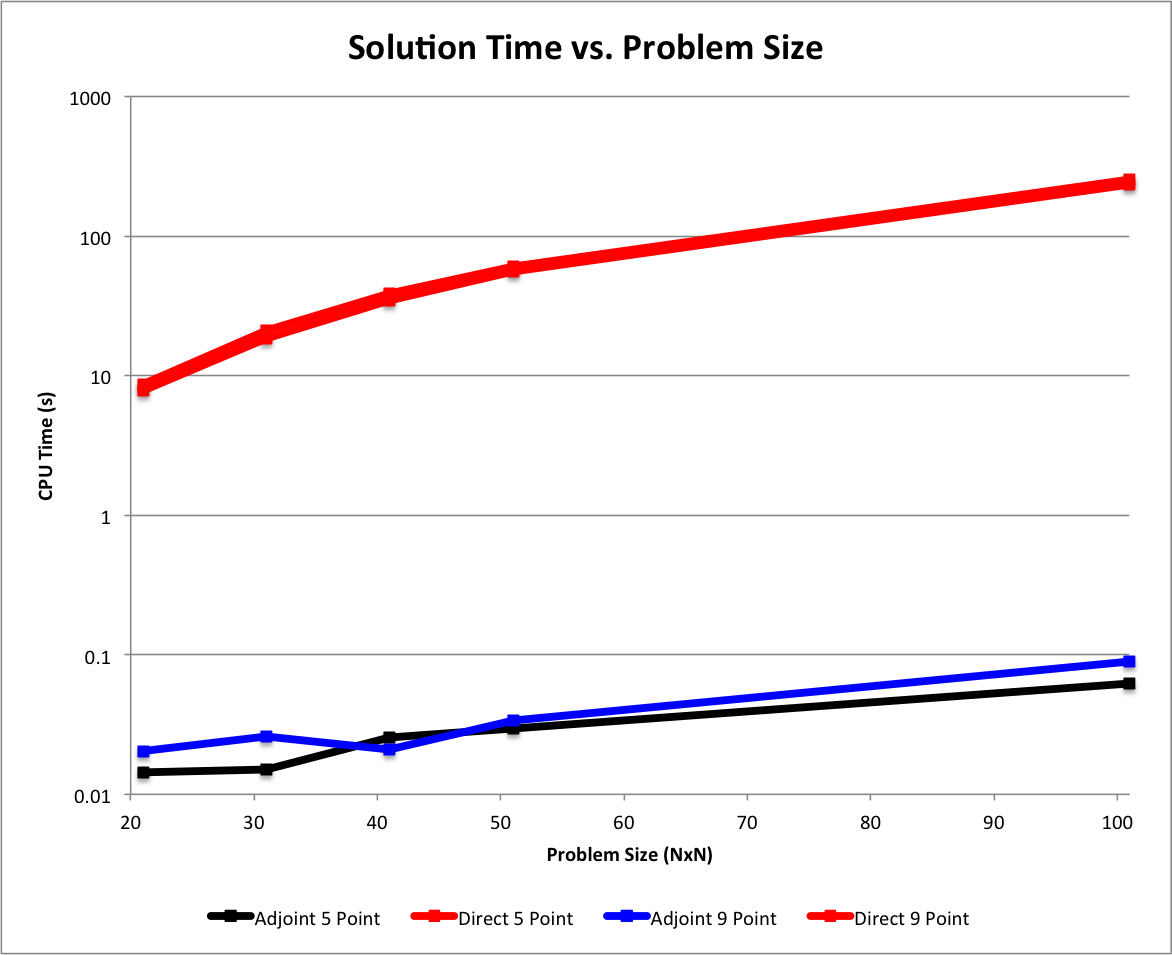
\includegraphics[width=5in]{AdjointDirectCPUTime.png}
  \caption{\sl CPU Time (s) to converge vs. Problem Size (N for an NxN
    problem). Both the adjoint and direct solvers are used with the
    five point and nine point stencils. A significant CPU time speedup
    is noted with the adjoint method due to the reduced number of
    histories.}
  \label{fig:cpu_time}
\end{figure}

\begin{figure}[htbp!]
  \centering
  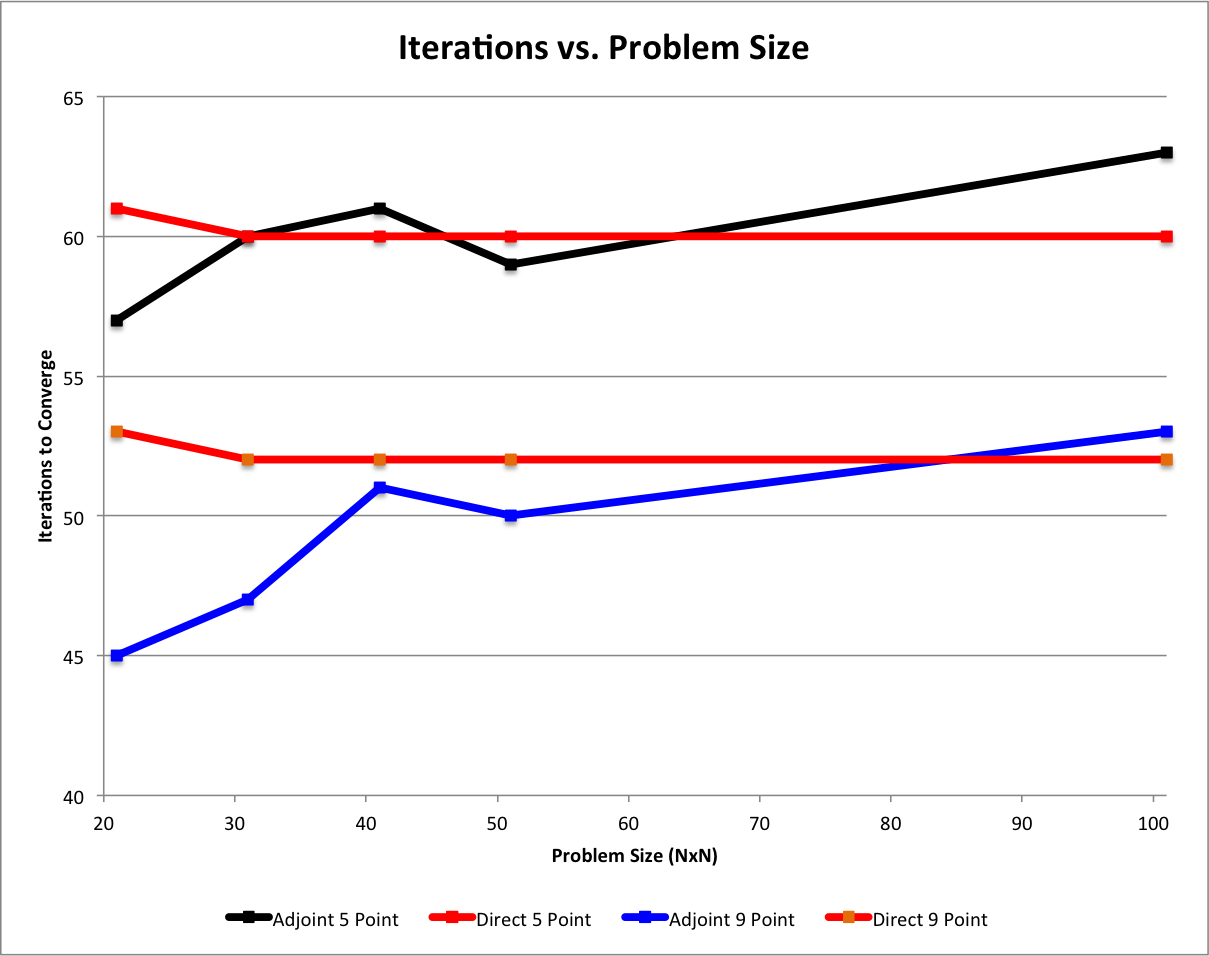
\includegraphics[width=5in]{AdjointDirectIterations.png}
  \caption{\sl Iterations to converge vs. Problem Size (N for an NxN
    problem). Both the adjoint and direct solvers are used with the
    five point and nine point stencils. Both methods give similar
    iteration behavior.}
  \label{fig:iterations}
\end{figure}

%%---------------------------------------------------------------------------%%
\section{Convergence Study Results}
Although CPU time was shown to be greatly decreased by using the
adjoint solver in the preceeding section, the iteration behavior was
approximately the same. To assess the convergence properties of MCSA
using each solver and stencil, the infinity norm of the residual
computed in Eq. \ref{eq:mcsa_step2} was computed at each iteration for
a fixed problem size. Fig. \ref{fig:convergence} gives the results of
these computuations. First, it is worthy to note on the semilog plot
that we are indeed achieving the expected exponential convergence from
MCSA. Second, we note that both the direct and adjoint methods have
approximately equivalent convergence behavior. Finally, it is observed
the the fourth-order accurate Laplacian stencil converges in fewer
iterations than the second-order accurate stencil as expected.

\begin{figure}[htpb!]
  \centering
  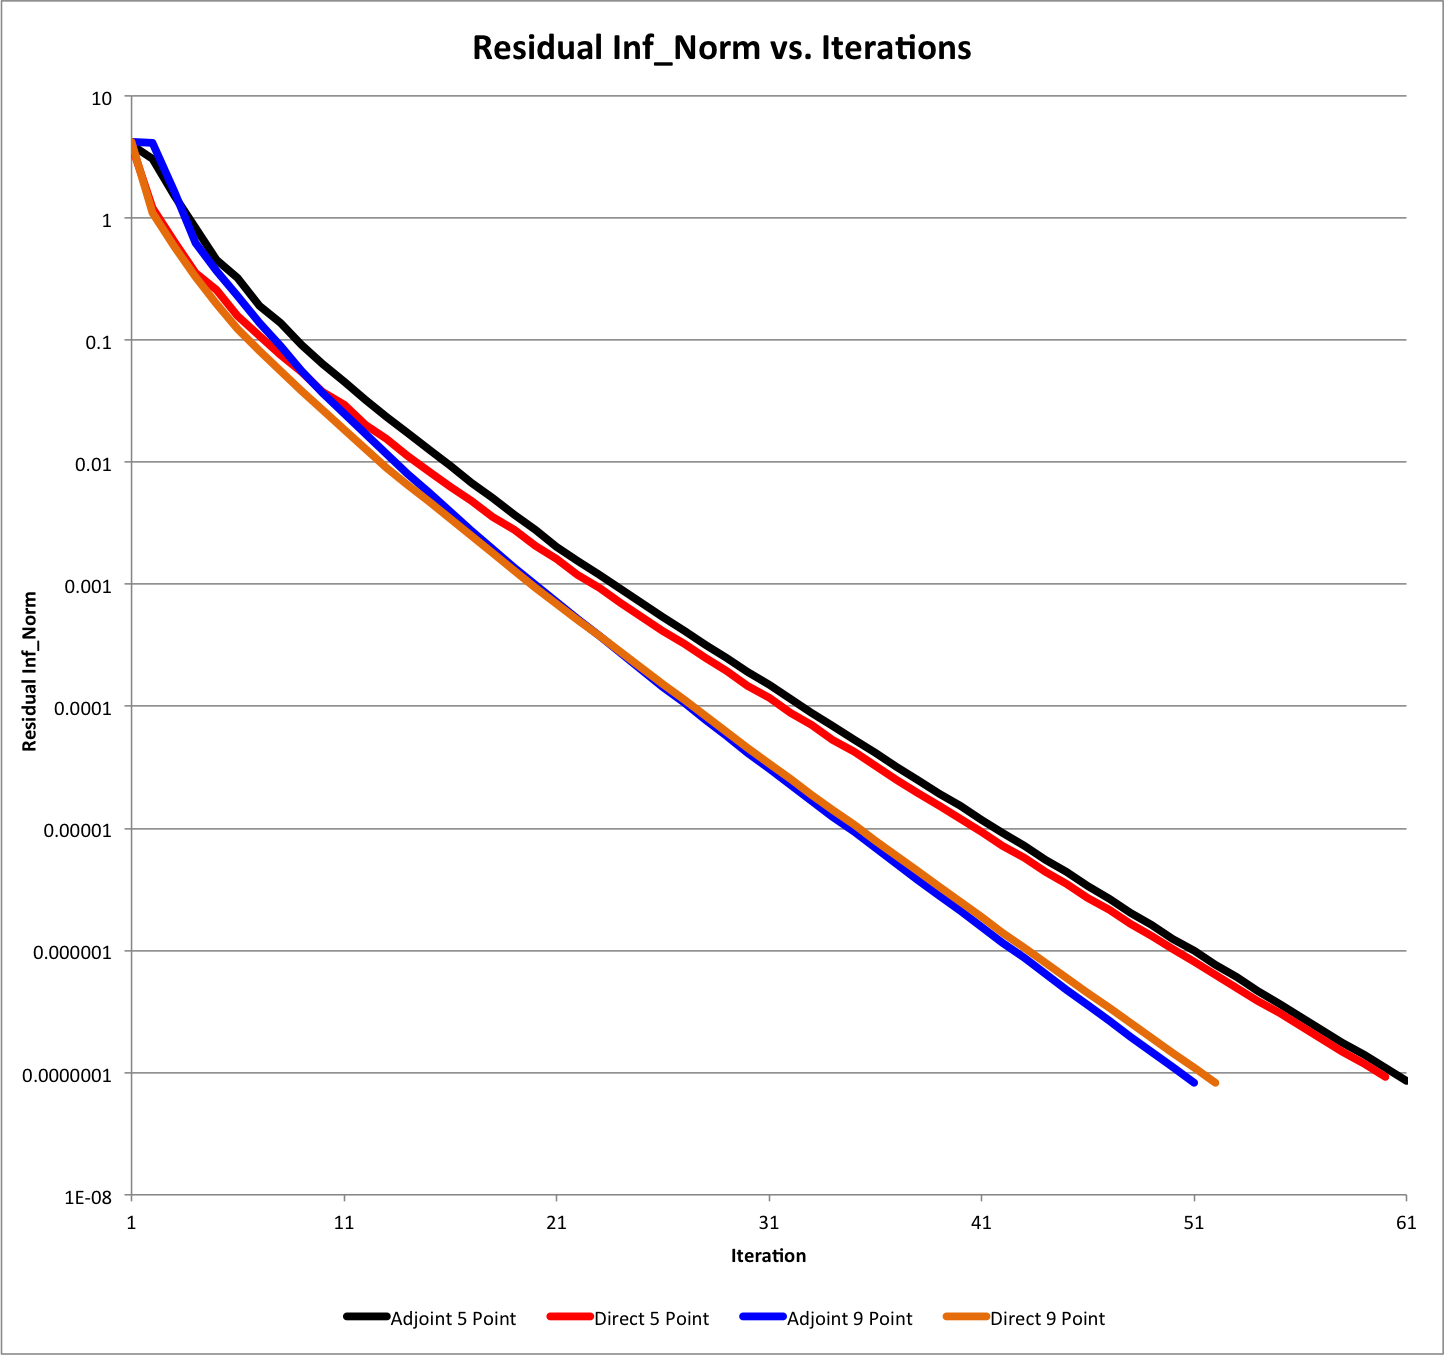
\includegraphics[width=5in]{AdjointDirectConvergence.png}
  \caption{\sl Infinity norm of the solution residual vs. iteration
    number for a problem of fixed size. Both the adjoint and direct
    solvers are used with the five point and nine point stencils. Both
    methods give similar iteration behavior.}
  \label{fig:convergence}
\end{figure}

%%---------------------------------------------------------------------------%%
\section{Conclusion}
A parameter study has been completed to verify that an adjoint
stochastic solver should be used with an MCSA implementation instead
of a direct stochastic solver. Several orders of magnitude reduction
in CPU time is observed when using the adjoint solver over the
direct. In addition, it was observed that MCSA had similar exponential
convergence properties with both the direct and adjoint solvers. Even
for cases where fewer iterations were needed to converge to a solution
using the direct solver, the large number of histories required caused
the CPU time to become large compared to the adjoint method.

%%---------------------------------------------------------------------------%%
%% BIBLIOGRAPHY STUFF

\bibliographystyle{rnotes}
\bibliography{direct_vs_adjoint}

\closing
\caution
\end{document}

%%---------------------------------------------------------------------------%%
%% end of direct_vs_adjoint.tex
%%---------------------------------------------------------------------------%%
